\fig{fv:c3:stationary}{同为水平切线，导数是否变号决定极值性质}{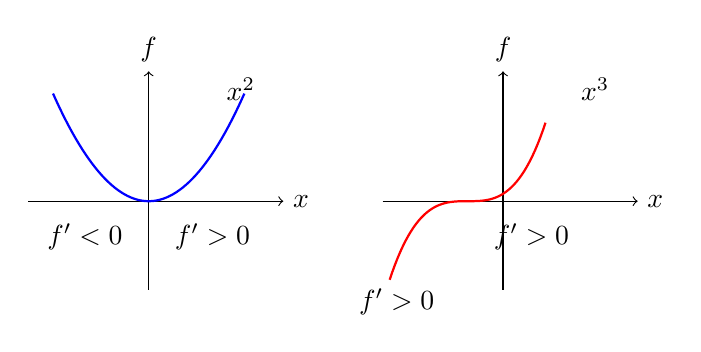
\begin{tikzpicture}[x=.9cm,y=.75cm]
\foreach \x/\lab in {0/{$x^2$},4.5/{$x^3$}}{\begin{scope}[xshift=\x cm]
\draw[->](-1.7,0)--(1.9,0)node[right]{$x$};\draw[->](0,-1.5)--(0,2.2)node[above]{$f$};\node at(1.3,1.9){\lab};\end{scope}}
\draw[blue,thick,domain=-1.35:1.35,samples=60]plot(\x,{\x*\x});
\draw[red,thick,domain=-1.1:1.1,samples=60]plot({4.5+\x},{\x*\x*\x});
\node at(-.9,-.6){$f'<0$};\node at(.9,-.6){$f'>0$};
\node at(3.5,-1.7){$f'>0$};\node at(5.4,-.6){$f'>0$};
\end{tikzpicture}}
图\ref{fv:c3:stationary}左图从原点左侧减小、右侧增大，原点确为极小点；右图经过原点仍递增，水平切线只表示瞬时斜率为零。因而解 $f'=0$是找候选点，读取两侧变化才完成判别。若自变量还限于闭区间，例如 $x^3$在 $[-1,1]$内求最值，最大、最小分别在端点，原点的驻点性质不能替代端点比较。
